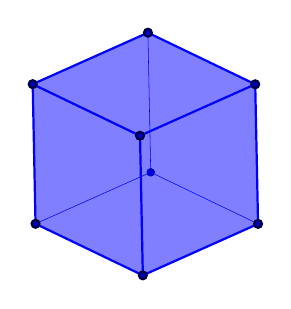
\begin{tikzpicture}%
	[x={(0.681462cm, -0.327528cm)},
	y={(0.731633cm, 0.326817cm)},
	z={(-0.017949cm, 0.886519cm)},
	scale=1.000000,
	back/.style={very thin},
	edge/.style={color=blue, thick},
	facet/.style={fill=blue,fill opacity=0.500000},
	vertex/.style={inner sep=1pt,circle,draw=blue!25!black,fill=blue!75!black,thick,anchor=base}]
%
%
%% Coordinate of the vertices:
%%
\coordinate (-1.00000, -1.00000, 1.00000) at (-1.00000, -1.00000, 1.00000);
\coordinate (-1.00000, 1.00000, 1.00000) at (-1.00000, 1.00000, 1.00000);
\coordinate (-1.00000, 1.00000, -1.00000) at (-1.00000, 1.00000, -1.00000);
\coordinate (1.00000, 1.00000, -1.00000) at (1.00000, 1.00000, -1.00000);
\coordinate (1.00000, 1.00000, 1.00000) at (1.00000, 1.00000, 1.00000);
\coordinate (1.00000, -1.00000, -1.00000) at (1.00000, -1.00000, -1.00000);
\coordinate (1.00000, -1.00000, 1.00000) at (1.00000, -1.00000, 1.00000);
\coordinate (-1.00000, -1.00000, -1.00000) at (-1.00000, -1.00000, -1.00000);
%%
%%
%% Drawing edges in the back
%%
\draw[edge,back] (-1.00000, 1.00000, 1.00000) -- (-1.00000, 1.00000, -1.00000);
\draw[edge,back] (-1.00000, 1.00000, -1.00000) -- (1.00000, 1.00000, -1.00000);
\draw[edge,back] (-1.00000, 1.00000, -1.00000) -- (-1.00000, -1.00000, -1.00000);
%%
%%
%% Drawing vertices in the back
%%
\node[vertex,back] at (-1.00000, 1.00000, -1.00000)     {};
%%
%%
%% Drawing the facets
%%
\fill[facet] (1.00000, -1.00000, 1.00000) -- (1.00000, 1.00000, 1.00000) -- (1.00000, 1.00000, -1.00000) -- (1.00000, -1.00000, -1.00000) -- cycle {};
\fill[facet] (1.00000, -1.00000, -1.00000) -- (-1.00000, -1.00000, -1.00000) -- (-1.00000, -1.00000, 1.00000) -- (1.00000, -1.00000, 1.00000) -- cycle {};
\fill[facet] (1.00000, -1.00000, 1.00000) -- (-1.00000, -1.00000, 1.00000) -- (-1.00000, 1.00000, 1.00000) -- (1.00000, 1.00000, 1.00000) -- cycle {};
%%
%%
%% Drawing edges in the front
%%
\draw[edge] (-1.00000, -1.00000, 1.00000) -- (-1.00000, 1.00000, 1.00000);
\draw[edge] (-1.00000, -1.00000, 1.00000) -- (1.00000, -1.00000, 1.00000);
\draw[edge] (-1.00000, -1.00000, 1.00000) -- (-1.00000, -1.00000, -1.00000);
\draw[edge] (-1.00000, 1.00000, 1.00000) -- (1.00000, 1.00000, 1.00000);
\draw[edge] (1.00000, 1.00000, -1.00000) -- (1.00000, 1.00000, 1.00000);
\draw[edge] (1.00000, 1.00000, -1.00000) -- (1.00000, -1.00000, -1.00000);
\draw[edge] (1.00000, 1.00000, 1.00000) -- (1.00000, -1.00000, 1.00000);
\draw[edge] (1.00000, -1.00000, -1.00000) -- (1.00000, -1.00000, 1.00000);
\draw[edge] (1.00000, -1.00000, -1.00000) -- (-1.00000, -1.00000, -1.00000);
%%
%%
%% Drawing the vertices in the front
%%
\node[vertex] at (-1.00000, -1.00000, 1.00000)     {};
\node[vertex] at (-1.00000, 1.00000, 1.00000)     {};
\node[vertex] at (1.00000, 1.00000, -1.00000)     {};
\node[vertex] at (1.00000, 1.00000, 1.00000)     {};
\node[vertex] at (1.00000, -1.00000, -1.00000)     {};
\node[vertex] at (1.00000, -1.00000, 1.00000)     {};
\node[vertex] at (-1.00000, -1.00000, -1.00000)     {};
%%
%%
\end{tikzpicture}